\section{Design}

\begin{figure}
    \centering
    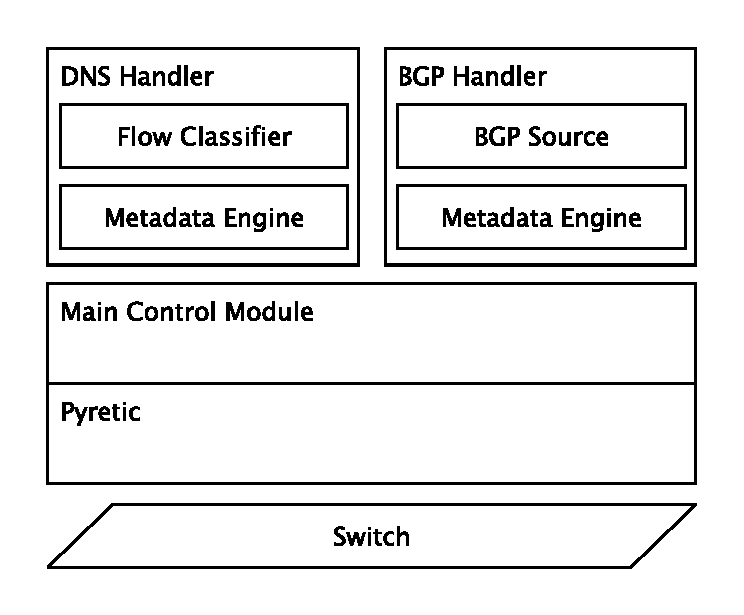
\epsfig{file=./diagrams/architecture2, width=.8\columnwidth}
%    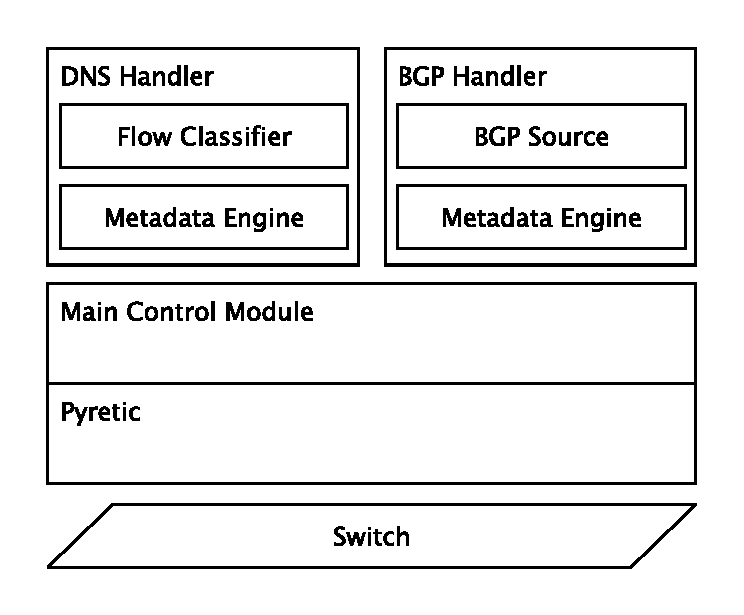
\epsfig{file=./diagrams/architecture2, width=1.0\columnwidth}
    \caption{\system{} architecture}
    \label{fig:architecture}
\end{figure}


\system{} is SDN-based system running on Pyretic~\cite{pyretic}, an easy to use and extend SDN programming language.
\system{} is divided into two sections, as can be seen in Figure~
\ref{fig:architecture}. These are the monitoring modules, two of which are described below, that provide traffic identification and monitoring information to the main control module (MCM). The MCM is responsible for combining the results from the monitoring modules, and triggering the reactive policies defined by the network operator.

\subsection{Monitoring Modules}
The monitoring modules perform two major functions: identifying flows that belong to a particular category and monitoring information related to that category. To identify flows, the modules can use information gleamed from monitoring network flows or from external data sources. The monitoring modules are designed such that new modules can be added in the future.

\subsection{DNS and BGP Handlers}
For the initial implementation, there are two modules being developed. Both are similar in design, but use different sources of information. The first, a DNS-based handler, will be described in detail, while the BGP-based handler will be quickly described.

The DNS handler which contains two parts, a flow classifier based on part of FlowQoS~\cite{FlowQoS} and a metadata engine. To perform flow classification, two pieces of information are needed: URL-to-classification mapping and IP-to-URL mapping. The URL-to-classification mapping is mentioned above where \tti{googlevideo.com} maps to `video'. This is a manual lookup, implemented as regular expression matching. The IP-to-URL mapping is based on monitoring DNS responses. At initialization, rules are installed at all ingress network devices to make a copy of DNS responses, forward one to the actual destination, and forward the second to the DNS handler. The flow classifier then extracts the domains and associated IP addresses, and uses the URL-to-classification mapping to determine what type of traffic is associated with a particular IP address. 
The metadata engine handles policy implementation for DNS-based classification. The metadata engine is responsible for breaking down the high-level policies passed from the MCM into the constituent components, and handling any changes that my occur dynamically (\ie{}, when a new DNS response comes in, or DNS response time-to-live (TTL) is reached). It is also responsible for aggregating data, such as aggregating the number of bytes transferred by video sources.

To go over the example above, if during the example above a DNS response from \tti{googlevideo.com} with associated IP of 198.51.100.8 was seen, the URL will be classified as video, and, as such, traffic coming from 198.51.100.8 would be classified as video. This will cause the \tti{matchClass} policy to generate a new \tti{match} action to run in parallel with any preexisting actions associated with video traffic. 

To allow for rules based on traffic related to a particular AS, BGP information is necessary. \system{} uses an external source of BGP information. This could be a connection to a local BGP server, or could be a static database of known routes. The BGP information source plays a similar role to the Flow Classifier in the DNS handler: it provides a lookup source for AS routes, and, more importantly, ranges of addresses controlled by a particular AS.

%Since BGP routes can update dynamically, the AS Handler handles these updates in much the same way as the BGP Handler handles expiration of DNS information. This allows for implementation the aforementioned security policy wherein ASes on blacklists can have their traffic redirected to a security appliance easily.


\begin{figure}
    \centering
%    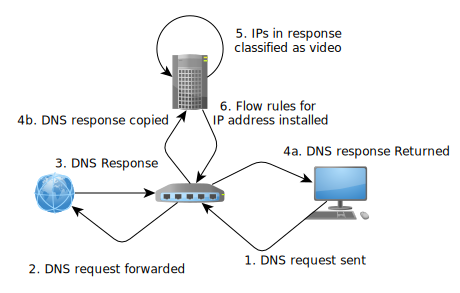
\epsfig{file=./diagrams/flow, width=.8\columnwidth}
    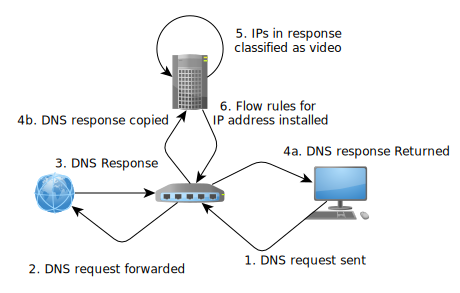
\epsfig{file=./diagrams/flow, width=1.0\columnwidth}
    \caption{Behavior of \system{}'s DNS handler classifying a video flow.}
    \label{fig:flow}
\end{figure}


